\begin{figure*}
    \centering
    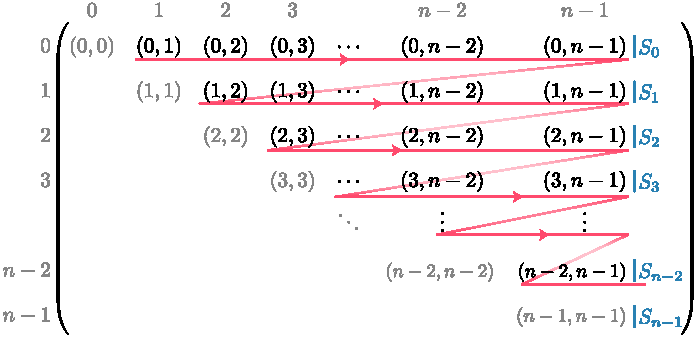
\includegraphics[width=0.7\textwidth]{assets/illustrator/traverse-schema.pdf}
    \caption{Row-major traversal of the adjacency matrix. $n$ is the total number of words (\ie nodes).}
    \label{fig:traverse-schema}
\end{figure*}

\section{Data Preparation}
\label{sec:data}

We use the \href{https://github.com/frodonh/french-words}{\textbf{french-words}} dataset \cite{data_french_words}, which contains 691,969 French words. The limitation to the French language is arbitrary; the method presented here can be applied to any language that has phonetic transcriptions available, simply by replacing the underlying dataset.

It is compiled from several sources including (among others) the Debian package \href{https://packages.debian.org/fr/sid/wfrench}{wfrench}, \href{http://www.lexique.org/}{Lexique 3.83} \cite{data_lexique}, the \href{https://infolingu.univ-mlv.fr/DonneesLinguistiques/Dictionnaires/telechargement.html}{DELA dictionary} \cite{data_dela} as well as the \href{https://github.com/hbenbel/French-Dictionary}{French-Dictionary} \cite{data_french_csv}. The words also contain \acrfull{pos} tagging information, \eg whether it is a noun, verb, adjective etc. It also comprises the usage frequency according to Lexique.org and Google Ngrams\footnote{We use the average of both sources (or just one if the other is missing).}.

Since the french-words dataset does not include phonetic transcriptions, we merge it with the \href{https://github.com/DanielSWolf/wiki-pronunciation-dict}{\textbf{wiki-pronunciation-dict}} \cite{data_pronunciation} extracted from the French \href{https://fr.wiktionary.org/}{Wiktionnaire} to obtain 611,786 words with their \gls{ipa} transcription\footnote{If multiple transcriptions for one word are available, we (arbitrarily) only store the first one to ease data handling.}. We validate the merged dataset by manually checking random samples of the words. While the dataset is of high quality, it does occasionnally contain errors in the transcriptions that we will not address here.

For usage in the Needleman–Wunsch algorithm, we extract all used phonetic \acrshort{ipa} symbols and assign integer IDs to them. For our examples, we obtain \autoref{tab:phonetic-encoding}. Note that we consider \textipa{/dZ/} as one symbol, even though it is a combination of \textipa{/d/} and \textipa{/Z/}. The same applies to \textipa{/tS/}. This is to account for the different pronunciation of the combined symbols compared to the individual ones.

% \vspace{-0.2em}

\begin{table}[H]
    \centering
    \begin{tabular}{lll}
    \toprule
    \textbf{Word} & \textbf{\acrshort{ipa}} & \textbf{Encoding} \\
    \midrule
    \textit{puissance} & \textipa{/p\textturnh is\~As/} & $[0,18,16,11,26,11]$ \\
    \textit{nuance} & \textipa{/n\textturnh\~As/} & $[29,18,26,11]$ \\
    \bottomrule
    \end{tabular}
    \caption{Example of two words with their phonetic transcription and encoding.}
    \label{tab:phonetic-encoding}
\end{table}
